%! TEX program = xelatex
%! TEX root = ../main.tex
%! TEX encoding = utf-8

%%%%%%%%%%%%%%%%%%%%%%%%%%%%%%%%%%%%%%%%%%%%%%%%%%%%%%%%%%%%%%%%%%%%%%
%
%  哈尔滨工程大学学位论文 XeLaTeX 模版 —— 正文文件 chap02.tex
%
%  版本:1.0.0
%  最后更新:
%  修改者:Leo LiWenhui lwh@hrbeu.edu.cn
%  修订者:
%  编译环境1:Ubuntu 12.04 + TeXLive 2013/2014
%  编译环境2:Windows 7/8  + TeXLive 2013/2014
%
%%%%%%%%%%%%%%%%%%%%%%%%%%%%%%%%%%%%%%%%%%%%%%%%%%%%%%%%%%%%%%%%%%%%%

\chapter{XeLaTeX环境配置}[Enverioment of XeLaTeX]
\label{chap02}

\TeX{}~可以在 Windows 、 Linux 以及 MacOS 等操作系统下运行,
鉴于大部分人都是使用 Windows 或 Linux 类操作系统,
本文主要介绍着两类操作系统下的 \TeX{} 工作环境配置。

\section{Windows~操作系统}[Windows System]

\subsection{安装配置}[Install and Config]
在 Windows 下可以使用的 \TeX{}套件有很多种,常用的有 C\TeX{}\footnote{C\TeX{} 套件已经不再更新,现在作为一个扩展包已经包含在 \TeX{}Live 中。}和 \TeX{}Live。
其中 C\TeX{}只能在 Windows 系统下使用,而 \TeX{}Live 则可以在 Windows 或 Linux 系统下使用。
这两个套件都可以在网上免费下载到,建议大家在 \href{https://tug.org/texlive/}{\TeX{}Live官方网站 https://tug.org/texlive/}下载最新版本的 \TeX{}Live 安装,
如果是使用光盘镜像安装,可以在安装完成后在线升级以更新宏包到最新版本。

\TeX{}Live 可以联网在线安装,也可以通过光盘安装,这两种安装方式基本相同,下面以在线安装方式进行介绍。

首先在 \href{https://tug.org/texlive/}{\TeX{}Live官方网站 https://tug.org/texlive/}下载最新版本的 \TeX{}Live 安装程序,该网站提供两种在线安装工具 \href{https://mirror.ctan.org/systems/texlive/tlnet/install-tl-windows.exe}{install-tl-windows.exe} 和\href{https://mirror.ctan.org/systems/texlive/tlnet/install-tl.zip}{install-tl.zip},前者下载后可以直接运行安装,后者需先解压然后再运行安装程序进行安装,这两种安装方式后续的安装过程一致,这里以使用install-tl.zip进行安装作说明。

下载install-tl.zip完成后先解压,然后执行解压后的 install-tl-windows.bat 批处理文件,运行后显示安装界面如图 \ref{fig:ins-tex} 所示:

\begin{figure}[htbp]
  \centering
  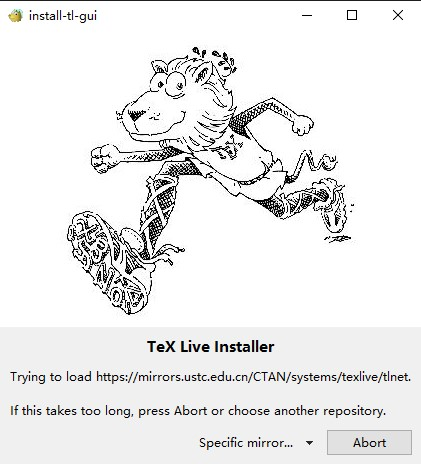
\includegraphics[scale=1.0]{install-texlive.jpg}
  \bicaption[fig:ins-tex]{}{\TeX{}Live安装}{Fig.}{Install \TeX{}Live}
\end{figure}

在线安装需要联网下载文件,可以通过点击 Specific mirror… $\blacktriangledown$ 从下拉列表中选择合适的镜像站点以提高下载、安装速度。当安装程序可以顺利链接所选站点下载安装文件后进入基本安装选项窗口,如图 \ref{fig:ins-bas} 所示:

\begin{figure}[htbp]
  \centering
  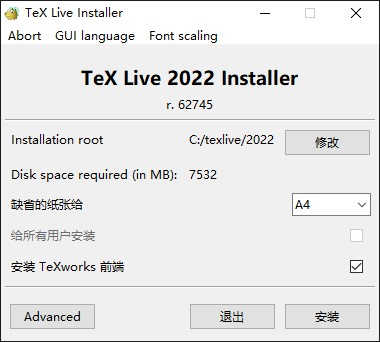
\includegraphics[scale=1.0]{install-basic.jpg}
  \bicaption[fig:ins-bas]{}{基本安装选项}{Fig.}{Basic install of \TeX{}Live}
\end{figure}

在基本按照选项窗口可以选择 \TeX{}Live 的安装位置、默认输出纸张大小等选项,一般情况下可以采用默认的安装选项直接点击【安装】按钮进行安装,也可以点击【Advanced】按钮进入高级安装界面(如图 \ref{fig:ins-adv})对实现更多的安装配置。

\begin{figure}[htbp]
  \centering
  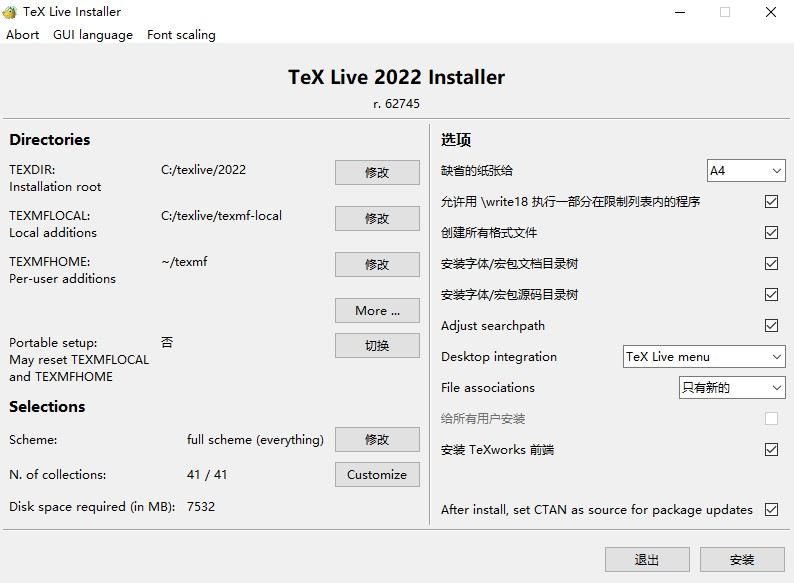
\includegraphics[width=\textwidth{},keepaspectratio]{install-advance.jpg}
  \bicaption[fig:ins-adv]{}{高级安装选项}{Fig.}{Advanced install of \TeX{}Live}
\end{figure}

点击【安装】按钮开始安装后,安装程序将自动完成数据下载、安装和环境配置等工作,根据网络情况,可能需要比较长的安装时间。

\subsection{编译运行}
\TeX{}Live 安装程序在安装完成后也会自动将程序路径加入到环境变量 PATH 中,方便用户使用。需要时用户也可自行修改 PTAH 环境变量。


默认的,\TeX{}Live安装包中会带有 TeXWorks 软件,这是一个非常不错的 \TeX{}编辑工具。

除了 TeXWorks 之外,还有很多其他优秀的编辑器可用于 tex 文件的编辑,例如 WinEdt、TeXStudio 等 ,当然也可以使用其他纯文本编辑器,例如记事本、Visual Studio Code、vim等。

以本模版为例,在 Windows 下使用 WinEdt 的编译过程是这样的:
\begin{enumerate}
  \item[(1)] 打开main.tex文件;
  \item[(2)] 先点击WinEdt工具栏上的\XeLaTeX{}按钮(可能在Acrobat Reader按钮的下拉菜单中);
  \item[(3)] 再点击WinEdt工具栏上的Bib\TeX{}按钮;
  \item[(4)] 再点击WinEdt工具栏上的\XeLaTeX{}按钮两到三遍;
  \item[(5)] 最后点击WinEdt工具栏上的Acrobat Reader按钮就可以看到输出的PDF文档了。
\end{enumerate}

\section{Linux~操作系统(以~Ubuntu~为例)}[Linux System]

\subsection{安装配置}[Install and Config]

首先的工作是安装一个合适的 \XeTeX{}编译系统。这个问题
并不难解决,现在主流的 \LaTeX{}编译系统均已经包含了对 \XeTeX{}的支持(包
括 xeCJK 中文宏包),并不需要自己额外再进行安装。在Linux下推荐使
用 \TeX{}Live ,目前最新版本为 \TeX{}Live 2022。下面以在 Ubuntu 下的本地安装为
例,简要的说明 \TeX{}Live 的安装及配置过程,高玩们请主动绕行:

\begin{enumerate}
  \item[(1)] 下载 \TeX{}live 2022 镜像,点击\href{https://tug.org/texlive/}{这里}进    入 \TeX{}live 2022 网站选择需要下载的安装文件或文档。
  \item[(2)] 安装 perl-tk 包,以便使用图形界面进行安装。在终端中输入命    令\texttt{sudo apt-get install perl-tk};
  \item[(3)] 挂载下载好的iso镜像,\texttt{sudo mkdir /mnt/texlive}(在~{/mnt}~下创建texlive文件夹),\texttt{sudo mount -o loop texlive2022.iso  /mnt/texlive}(挂载texlive2022.iso)。进入~/mnt/texlive~目录,输入命令~\texttt{sudo ./install-tl -gui}~之后出现图形界面。之后的操作就比较简单了,可以去掉不用的语言包以节省磁盘空间,注意选择最后一项 Create symlinks in system directories ,让安装程序自动创建语法链接。确定安装,耐心等待进度条到头;
  \item[(4)] 配置环境变量。在终端中输入~\texttt{sudo gedit /etc/bash.bashrc},在此文件末尾添加
\end{enumerate}

\begin{lstlisting}
    PATH=/usr/local/texlive/2022/bin/i386-linux: $PATH;
    export PATH
    MANPATH=/usr/local/texlive/2022/texmf/doc/man: $MANPATH;
    export MANPATH
    INFOPATH=/usr/local/texlive/2022/texmf/doc/info: $INFOPATH;
    export INFOPATH
  \end{lstlisting}

在~{/etc/manpath.config}~文件的~\texttt{set up PATH to  MANPATH mapping}~这行下面的列表后增加一条:

\begin{lstlisting}
    MANPATH_MAP /usr/local/texlive/2022/bin/i386-linux  /usr/local/texlive/2022/texmf/doc/man
  \end{lstlisting}

在~{/etc/manpath.config}~文件的~\texttt{set up PATH to  MANPATH mapping}~这行下面的列表后增加一条:

\begin{lstlisting}
    MANPATH_MAP /usr/local/texlive/2022/bin/i386-linux /usr/local/texlive/2022/texmf/doc/man
  \end{lstlisting}

至此安装过程结束。

如果是在 Windows 系统下,可直接将 Texlive 可执行文件加入系统 PATH 环境变量中。

之后我们需要一个类似于 WinEdt 或 TeXStudio 的集成编译环境。在 Ubuntu 软件中心中,我们能很
容易的安装 \TeX{}maker 和 \TeX{}works ,两者功能差不多, \TeX{}maker 更强大一些。
当然,你也可以自己配置 VIM 下的 \LaTeX{}编译环境。在 Windows 环境下,可以在网上下载免费的
TeXStudio 软件进行 tex 文件编辑。

\subsection{生成论文}[Compile]
\label{sec:generate-thesis}

在安装并配置好编译环境之后,接下来的工作就是如何编译 \XeLaTeX{} 文件,生成
所需的 PDF 文档了。

任何文本编辑工具都可以用来编写论文,当然 Linux 下也有很多免费的集成编辑工具可以使用。

本节介绍几种常见的生成论文的方法。用户可根据自己的情况选择。

\subsubsection{\XeLaTeX}
\label{sec:xelatex}

很多用户对 \LaTeX\ 命令执行的次数不太清楚。一个基本的原则是多次运行 \LaTeX\ 命
令直至不再出现警告。下面给出生成示例文档的详细过程(\texttt{\#} 开头的行为注
释),首先来看推荐的 \texttt{xelatex} 方式:

(1) 发现里面的引用关系,文件后缀 .tex 可以省略

\begin{lstlisting}
    $ xelatex main
\end{lstlisting}

(2) 编译参考文件源文件,生成 bbl 文件

\begin{lstlisting}
    $ bibtex main
\end{lstlisting}

(3) 解决引用

\begin{lstlisting}
    $ xelatex main
    $ xelatex main   # 如果不需要生成索引此时生成完整的 pdf 文件
    $ splitindex main -- -s heuthesis.ist  # 自动生成索引
    $ xelatex main.tex
\end{lstlisting}

\subsubsection{latexmk}
\label{sec:latexmk}

\texttt{latexmk} 命令支持全自动生成 \LaTeX\ 编写的文档,并且支持使用不同的工具
链来进行生成,它会自动运行多次工具直到交叉引用都被解决。下面给出了一个用
\texttt{latexmk} 调用 \texttt{xelatex} 生成最终文档的示例:

\begin{lstlisting}
    $ latexmk -xelatex main
\end{lstlisting}

\subsubsection{make}
\label{sec:make}

上面使用 \texttt{xelatex} 生成论文的方法虽然不复杂,但是每次都输入还是非常罗嗦,所以 \heuthesis\
提供了一个 \texttt{Makefile},可以通过在命令行环境下执行一次 make 完成论文生成这些工作。

\subsubsection{buidl.bat}
\label{sec:build}

示例文件夹中也包含了 \texttt{build.bat} 批处理文件,在 \texttt{Windows} 环境下可以
直接使用改批处理文件生成最终 \texttt{PDF} 格式的论文 \texttt{main.pdf}。

\subsection{原创性和授权声明}
\label{sec:generate-auth}

按学校研究生论文规范要求,硕士和博士论文扉页后应有论文原创性和授权声明签字页。
该页可以使用两种方式实现:

\begin{enumerate}
  \item[(1)] \texttt{\cs authorization}
  \item[(2)] \texttt{\cs authorization[auscan.pdf]}
\end{enumerate}

格式(1)不带参数,使用模板生成的空白原创性和授权声明签字页,可先使用这种方式生成签字页后进行打印签字,然后扫描成 PDF 格式文件。

格式(2)使用带参数的方式,~\texttt{[auscan.pdf]}~指定使用~\texttt{auscan.pdf}~文件作为嵌入到论文中的原创性和授权声明签字页。

模板目录中已包含空白论文原创性和授权声明文件 auscan.pdf,可以在生成论文前使用签字后扫描的pdf文件进行替换,也可以指定其他符合系统要求的文件名称。

\subsection{生成封面}
\label{sec:generate-cover}

模板还提供了用于生成论文 \texttt{A3} 页面的封面定义文档。用户可根据自己的情况选择。

A3 封面的生成是利用上述论文的首页封面和书脊拼合而成,因此在生成 A3 封面前
需要先生成论文 \texttt{main.pdf} 并在 \texttt{spine.tex} 定义论文标题和作者姓名信息,
然后使用 \texttt{xelatex} 依次编译 \texttt{spine.tex} 和 \texttt{a3cover.tex}:

(1)使用 xelatex

\begin{lstlisting}
    $ xelatex spine
    $ xelatex a3cover
\end{lstlisting}

(2)或者使用 latexmk

\begin{lstlisting}
    $ latexmk spine
    $ latexmk a3cover
\end{lstlisting}

在 \texttt{Windows} 系统下也可以直接使用 \texttt{make\_cover.bat} 批处理生成 \texttt{A3} 封面。

\section{字库安装}[Font Install]

可以通过模板选项选择~\texttt{fontset}~使用Windows系统字体或者Adobe字体。

本模板默认是使用Windows字体字库,可以不用设置字体选项,如果使用Adobe字体字库,需要设置~\texttt{fontset=adobe}~。
在使用此模板撰写论文前,应该确保相应的字库已经安装,并且最好是包含宋体、黑体、楷体和仿宋的完整套装。

在 Windows 操作系统下,只要把字库文件复制到 Windows 的 Fonts 文件夹下即可,
而对于 Linux 系统,可通过右键点击字库文件然后选择【安装字库】菜单选项进行安装。
Linux 对于系统新安装的字库,需要使用命令~\texttt{sudo fc-cache -fsv}~刷新缓存后才可以使用。

\section*{本章小结}[Brief Summary]
\LaTeX{}~工作环境安装与配置简介。
